\begin{figure}[htbp]
\centering
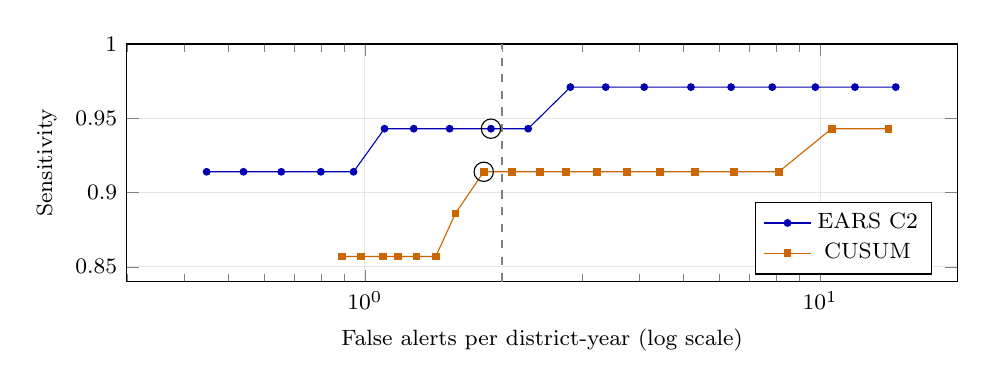
\begin{tikzpicture}
\begin{axis}[width=\columnwidth, height=4.6cm, xmode=log, log basis x=10, xmin=0.3, xmax=20, ymin=0.84, ymax=1.0,
  xlabel={False alerts per district-year (log scale)}, ylabel={Sensitivity}, legend pos=south east,
  legend style={font=\footnotesize}, tick label style={font=\footnotesize}, label style={font=\footnotesize},
  grid=major, grid style={gray!20}]
\addplot[mark=*, mark size=1.2pt, blue!70!black] coordinates {(0.449,0.914) (0.541,0.914) (0.655,0.914) (0.8,0.914) (0.944,0.914) (1.104,0.943) (1.28,0.943) (1.535,0.943) (1.892,0.943) (2.283,0.943) (2.827,0.971) (3.381,0.971) (4.107,0.971) (5.202,0.971) (6.375,0.971) (7.851,0.971) (9.762,0.971) (11.925,0.971) (14.66,0.971)};
\addlegendentry{EARS C2}
\addplot[mark=square*, mark size=1.2pt, orange!80!black] coordinates {(0.892,0.857) (0.981,0.857) (1.095,0.857) (1.181,0.857) (1.298,0.857) (1.431,0.857) (1.581,0.886) (1.824,0.914) (2.107,0.914) (2.427,0.914) (2.76,0.914) (3.236,0.914) (3.769,0.914) (4.442,0.914) (5.301,0.914) (6.47,0.914) (8.116,0.914) (10.599,0.943) (14.13,0.943)};
\addlegendentry{CUSUM}
\draw[dashed, gray] (axis cs:2,0.84) -- (axis cs:2,1.0);
\addplot[only marks, mark=o, mark size=3.5pt, black, forget plot] coordinates {(1.892,0.943) (1.824,0.914)};
\end{axis}
\end{tikzpicture}
\caption{Detection trade-off (conflict C1): every setting of the sweep, the two-alert limit dashed, the chosen
settings circled.}
\label{fig:tradeoff}
\end{figure}
